\documentclass{article}
\usepackage{graphicx, fancyhdr, amsmath}
\usepackage[margin=0.6in, top=1in]{geometry}
\usepackage{float}
\usepackage[absolute, overlay]{textpos}
\usepackage[colorlinks=true, linkcolor=blue]{hyperref}

\pagestyle{fancy}
\fancyhf{}
\renewcommand{\headrulewidth}{0pt}

\fancyhead[L]{
\begin{textblock*}{2cm}(0.3in,0.1in)  % {block width} (x-coordinate, y-coordinate)
    
\includegraphics[width=2cm]{NEW LOGO.png}  % Example image placeholder
\end{textblock*}
}
\fancyhead[R]{Math Success Program, UCLA}
\fancyfoot[R]{Created for the MSP by Asmi Kawatkar}

\fancypagestyle{plain}{
}


\title{Review Sheet: Chain Rule, Product Rule, Quotient Rule}
\date{}
\author{}

\begin{document}
\maketitle
\vspace{-0.75in}
\section*{Content Review}
\subsection*{Overview}

\textit{Product Rule}: 
$$\frac{d}{dx} f(x) \cdot g(x) = f'(x) \cdot g(x) + g'(x) \cdot f(x)$$

\noindent Product Rule is sometimes also written as:

$$y = u\cdot v \Longrightarrow \frac{dy}{dx} = u \frac{dv}{dx} + v \frac{du}{dx} = v'u + u'v   \text{  where u,v are both functions in terms of x}$$

\noindent \textbf{Common Mistake:} Don't try to take the derivative of expressions like $y = 8x$ using product rule. This will be a normal derivative the way you have learned so far. Don't try to make constants (like 8) functions of x, this will only lead to confusion. 

\noindent \newline \textit{Quotient Rule}:
$$\frac{d}{dx}\frac{f(x)}{g(x)} = \frac{f'(x)g(x) - g'(x)f(x)}{(g(x))^2}$$

\noindent Quotient Rule is sometimes also written as:
$$y = \frac{u}{v} \Longrightarrow \frac{dy}{dx} = \frac{u'v - v'u}{v^2} \text{   where u,v are both functions in terms of x}$$

\noindent Quotient rule is essentially a special case of product rule where one of the functions has the power (-1), i.e $y = u\cdot v^{-1}$. If correctly applied, product rule can be used to derive quotient rule. However, at this level, it is just easier to remember the quotient rule. 

\noindent\newline 
\textit{Chain Rule}: The Chain Rule is probably one of the most important parts of fundamental calculus that you will learn. This idea will continue to appear at different places in engineering, mathematics, biology, chemistry, economics or other coursework. 

\noindent In simple terms, the chain rule can be stated as:

$$\frac{dy}{dx} = \frac{dy}{dm} \times \frac{dm}{dx}$$

\noindent The main idea here is the presence of the same variable (in this case m) on the diagonal. As long as you take the derivative of $y$ with respect to $m$, and take the derivative of $m$ with respect to $x$ separately, you can find the expression for $\frac{dy}{dx}$ without having to explicitly find $y$ in terms of $x$. 

\noindent 
\newline
This idea can also be extended to multiple levels of 'chains'. For instance:

$$\frac{dy}{dx} = \frac{dy}{dm} \times \frac{dm}{dt}\times\frac{dt}{dw}\times\frac{dw}{dx}$$

\noindent Once you learn to recognize this pattern of having the same variables on the 'diagonal', you will find chain rule to be more intuitive. 

\noindent 
\newline\textbf{For example:}
$$y = 4m^2 \text{ and } m = \sin{x} \text{, then we can find } \frac{dy}{dm} = 8m \text{ and } \frac{dm}{dx} = \cos x$$

By applying chain rule:

$$\frac{dy}{dx} = \frac{dy}{dm} \times \frac{dm}{dx} = 8m \cdot \cos x = 8(\sin x) \cdot \cos x = 8\sin x \cos x$$

Skip to \hyperref[WorkedProblems]{Worked Problems}
\subsection*{Resources}
\textit{Chain Rule}
\begin{itemize}
    \item \href{https://www.khanacademy.org/math/ap-calculus-ab/ab-differentiation-2-new/ab-3-1a/v/chain-rule-introduction}{Video: Chain Rule (Khan Academy, 5 min)}
    \item \href{https://youtu.be/HaHsqDjWMLU}{Video: Chain Rule for Finding Derivatives - with Worked Examples (Organic Chemistry Tutor, 20 min)}
    \item \href{https://www.rcboe.org/cms/lib/GA01903614/Centricity/Domain/9329/Practice-%20Chain%20Rule.pdf}{Worksheet: Chain Rule (has solutions)}
    \item \href{https://s3.amazonaws.com/calculus-worksheets/calculus-1-tutor/Calculus+1+Tutor+-+Worksheet+5+-+The+Chain+Rule.pdf}{Worksheet: Chain Rule (has worked solutions)}
\end{itemize}

\noindent \newline
\textit{Product Rule}
\begin{itemize}
    \item \href{https://www.khanacademy.org/math/ap-calculus-ab/ab-differentiation-1-new/ab-2-8/v/applying-the-product-rule-for-derivatives}{Video: Product Rule (Khan Academy, 3 min)} 

    \item \href{https://youtu.be/17X5g9QArTc}{Video: Product Rule for Derivatives - with Worked Examples}

    \item \href{https://tutorial.math.lamar.edu/problems/calci/productquotientrule.aspx}{Practice Problems: Product \& Quotient Rule (with Worked Solutions)}

    \item \href{https://cdn.kutasoftware.com/Worksheets/Calc/03%20-%20Product%20Rule.pdf}{Practice Problems: Product Rule (Worked Solutions)}

    \item \href{https://www.mathcentre.ac.uk/resources/uploaded/mc-ty-chain-2009-1.pdf}{Explainer Worksheet (Detailed Concept + Worked Examples)}
\end{itemize}

\noindent
\textit{Quotient Rule}
\begin{itemize}
    \item \href{https://www.khanacademy.org/math/ap-calculus-ab/ab-differentiation-1-new/ab-2-9/v/quotient-rule}{Video: Quotient Rule (Khan Academy, 4 min)}

    \item \href{https://youtu.be/8jVDEcQ0wXk}{Video: Quotient Rule for Derivatives - with Worked Examples (Organic Chemistry Tutor, 12 min)}

    \item \href{https://www.math.ucdavis.edu/~kouba/CalcOneDIRECTORY/quotientruledirectory/QuotientRule.html}{Practice Problems: Quotient Rule - with Worked Solutions (UC Davis Math)}
\end{itemize}

\subsection*{Acknowlegement}
Questions in the Worked Problems section of this sheet have been taken from external sources that have been linked where appropriate. All solutions have been developed independently. 

\pagebreak
\section*{Worked Problems}
\label{WorkedProblems}

\subsection*{Chain Rule}
Find the derivatives of the following functions (with respect to x):
\\ \href{https://mryangteacher.weebly.com/uploads/7/7/0/2/7702250/2.4_chain_rule_practice_ws_1.pdf}{Source} and another \href{https://tajimasolis.weebly.com/uploads/3/7/3/4/37346235/chain_rule_worksheet_1_and_2.pdf}{Source}

\begin{enumerate}
    \item $y = (5x+8)^4$
    \begin{figure}[H]
        \centering
        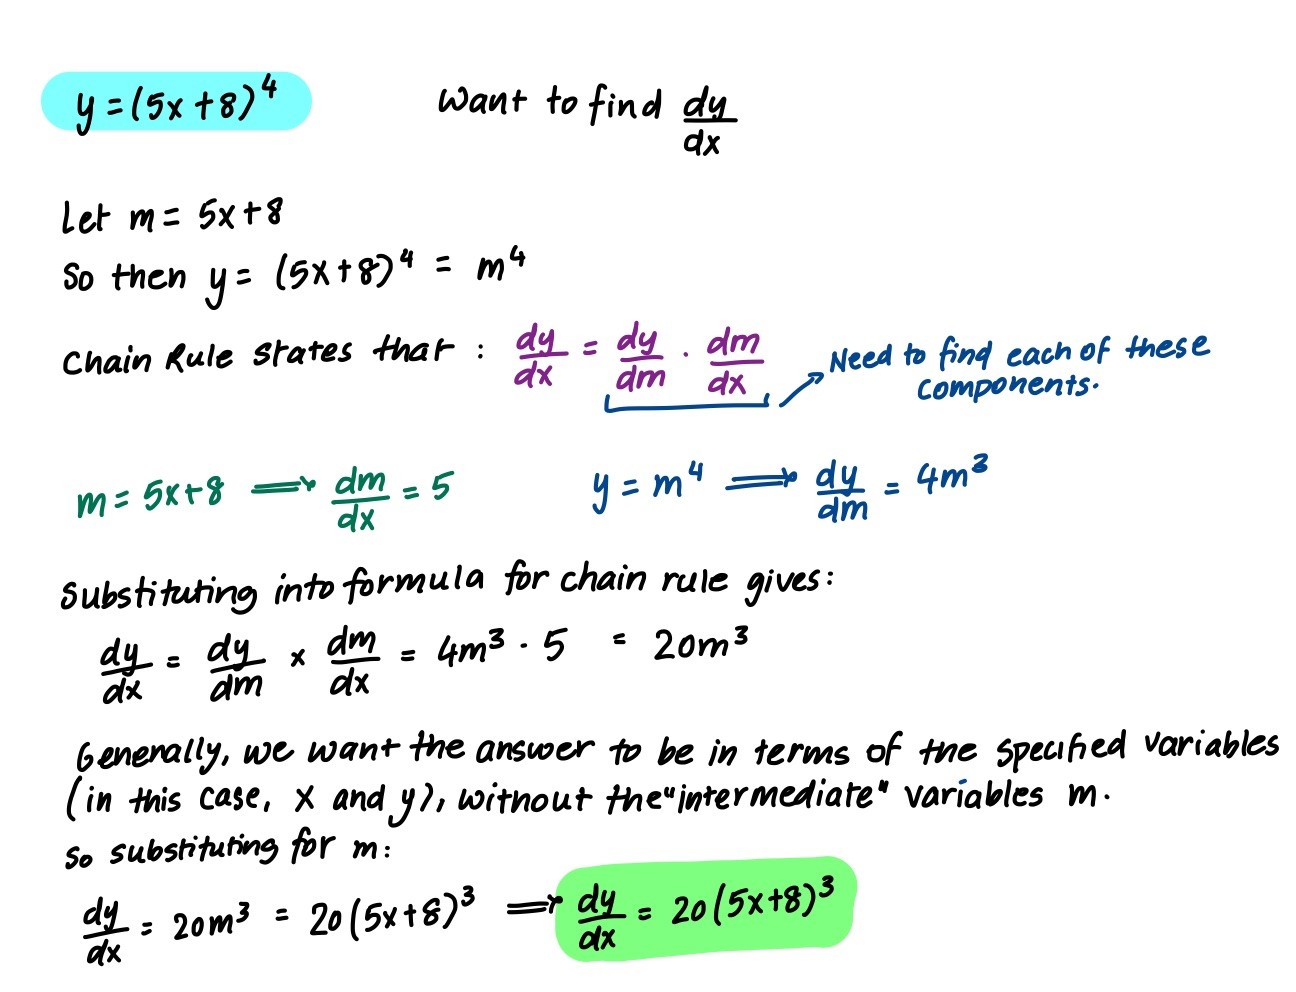
\includegraphics[width=0.78 \linewidth]{Q1.jpg}
        \label{fig:Q1}
    \end{figure}
    \item $y = 2(9-x^2)^\frac{1}{4}$
    \begin{figure}[H]
        \centering
        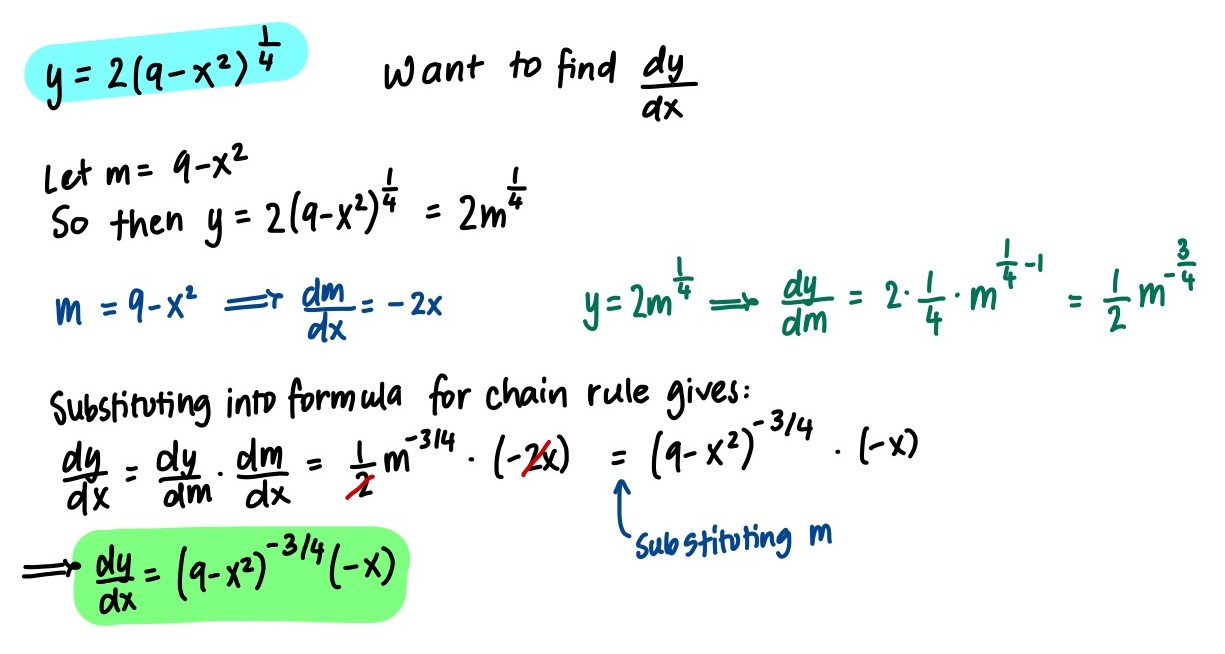
\includegraphics[width=0.78 \linewidth]{Q2.jpg}
        \label{fig:Q2}
    \end{figure}
    \item $y = \sqrt{x^2 -4x + 2}$
    \begin{figure}[H]
        \centering
        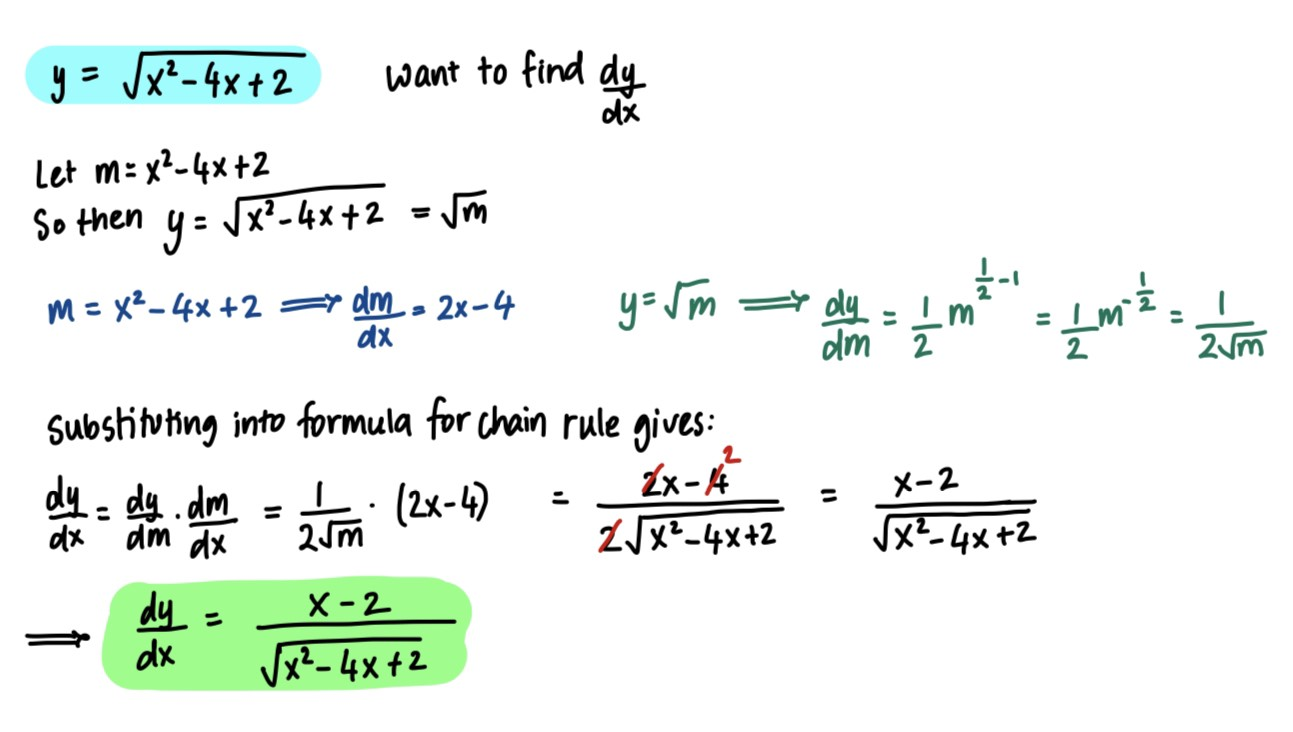
\includegraphics[width=0.7 \linewidth]{Q3.jpg}
        \label{fig:Q3}
    \end{figure}
    \item $y = \sin ^3 x + \cos^3 x$
    \begin{figure}[H]
        \centering
        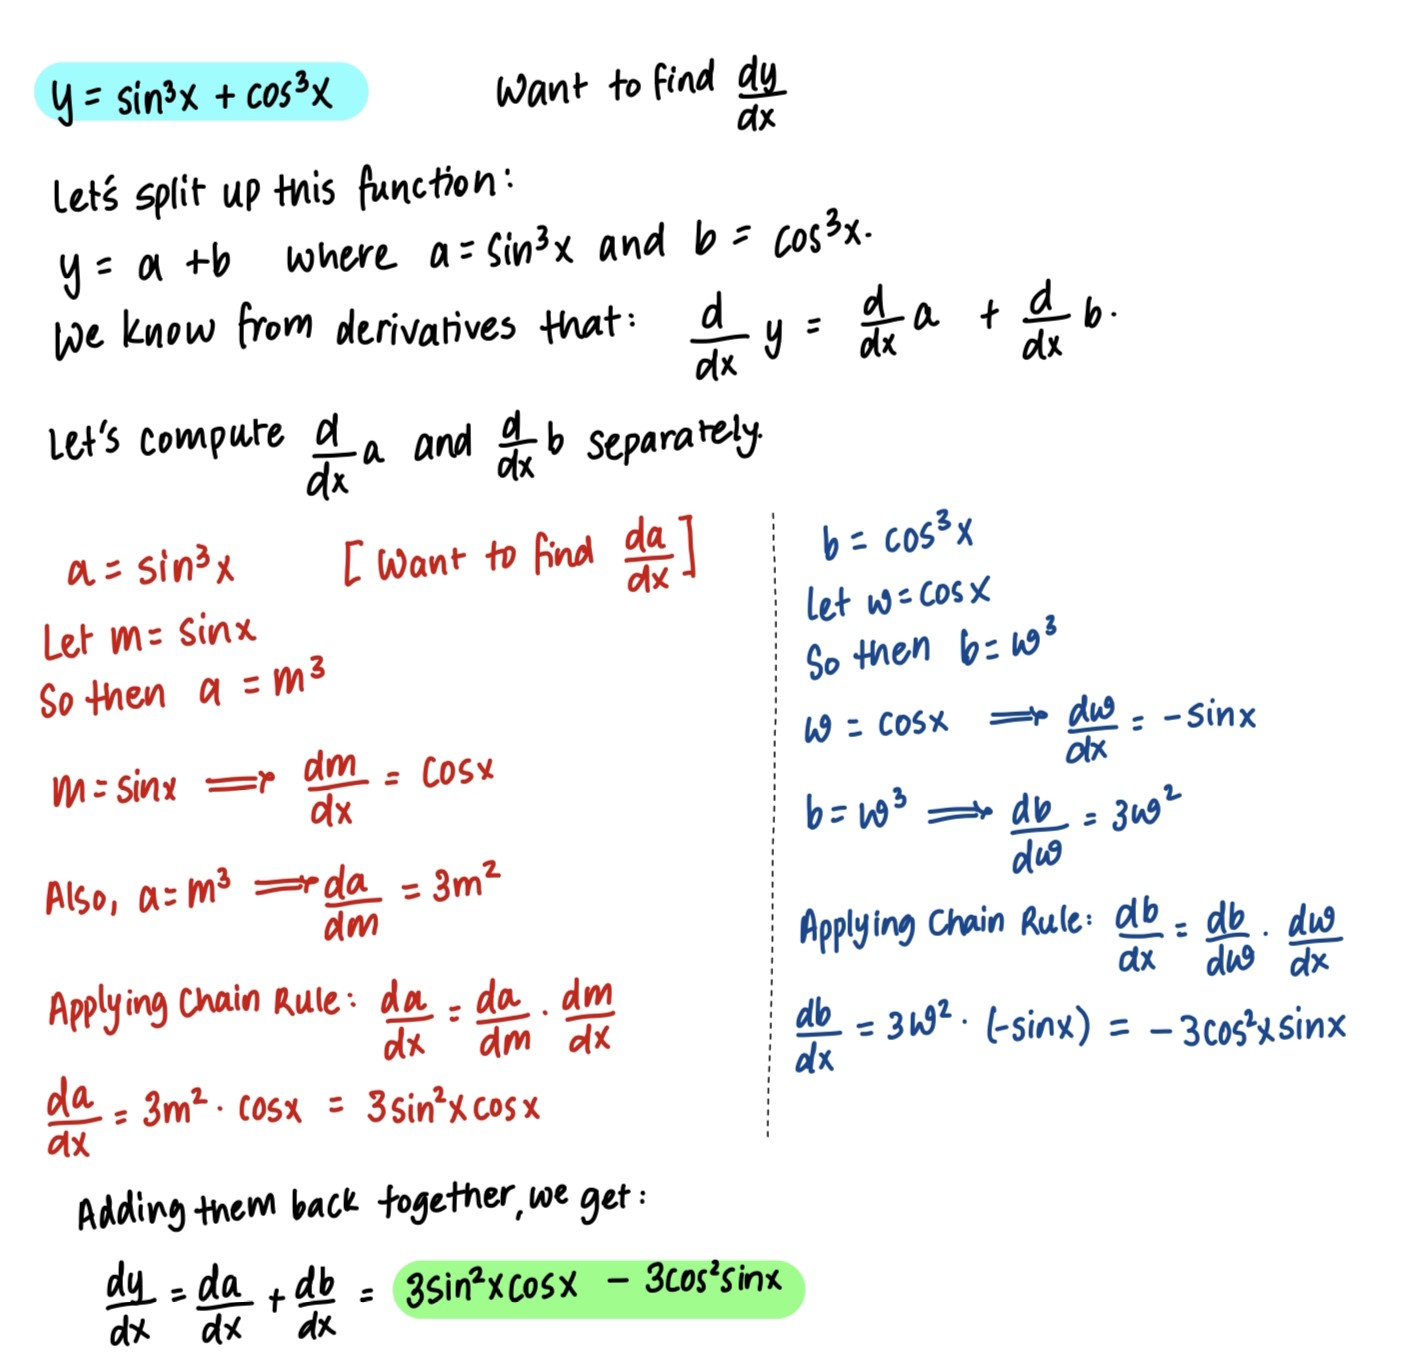
\includegraphics[width=0.78 \linewidth]{Q4.jpg}
        \label{fig:Q4}
    \end{figure}
    \item $y = \sin^2\left(\cos^4 x\right)$
    \begin{figure}[H]
        \centering
        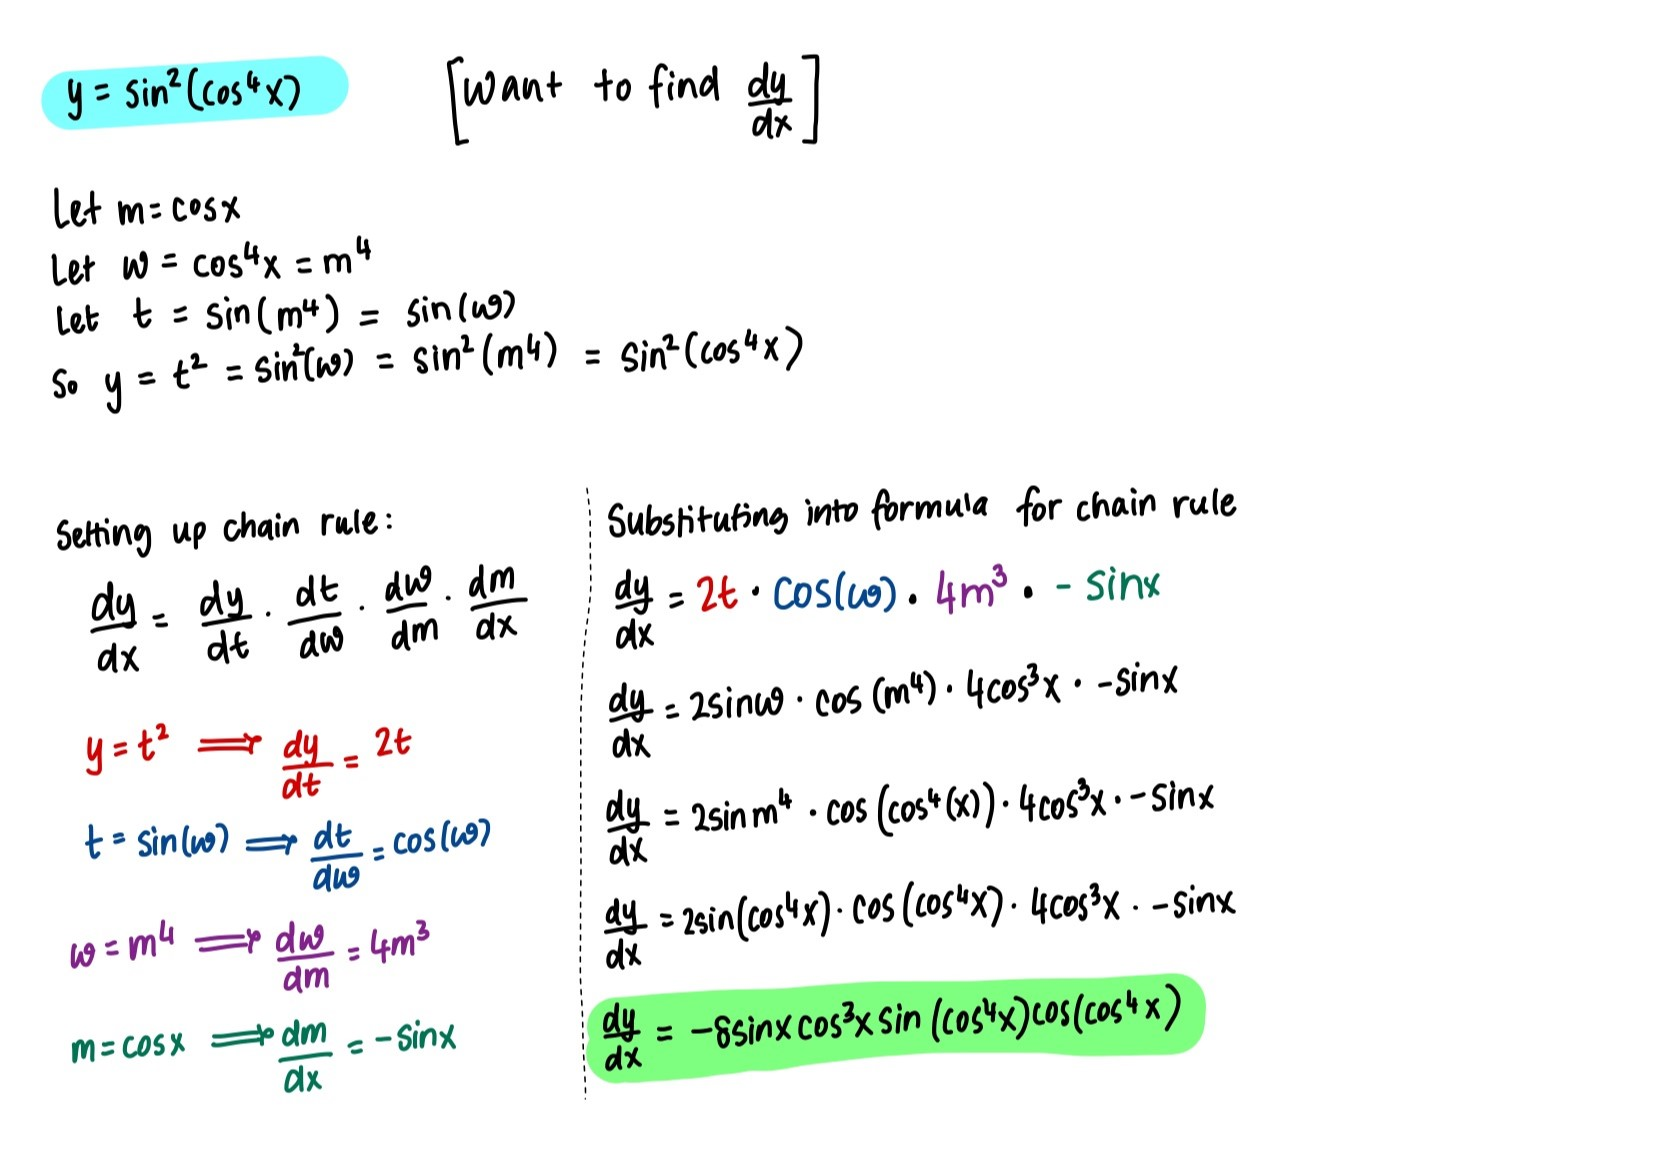
\includegraphics[width= \linewidth]{Q5.jpg}
        \label{fig:Q5}
    \end{figure}
    \item $y = \sin^3\left(2x+3\right)$
    \begin{figure}[H]
        \centering
        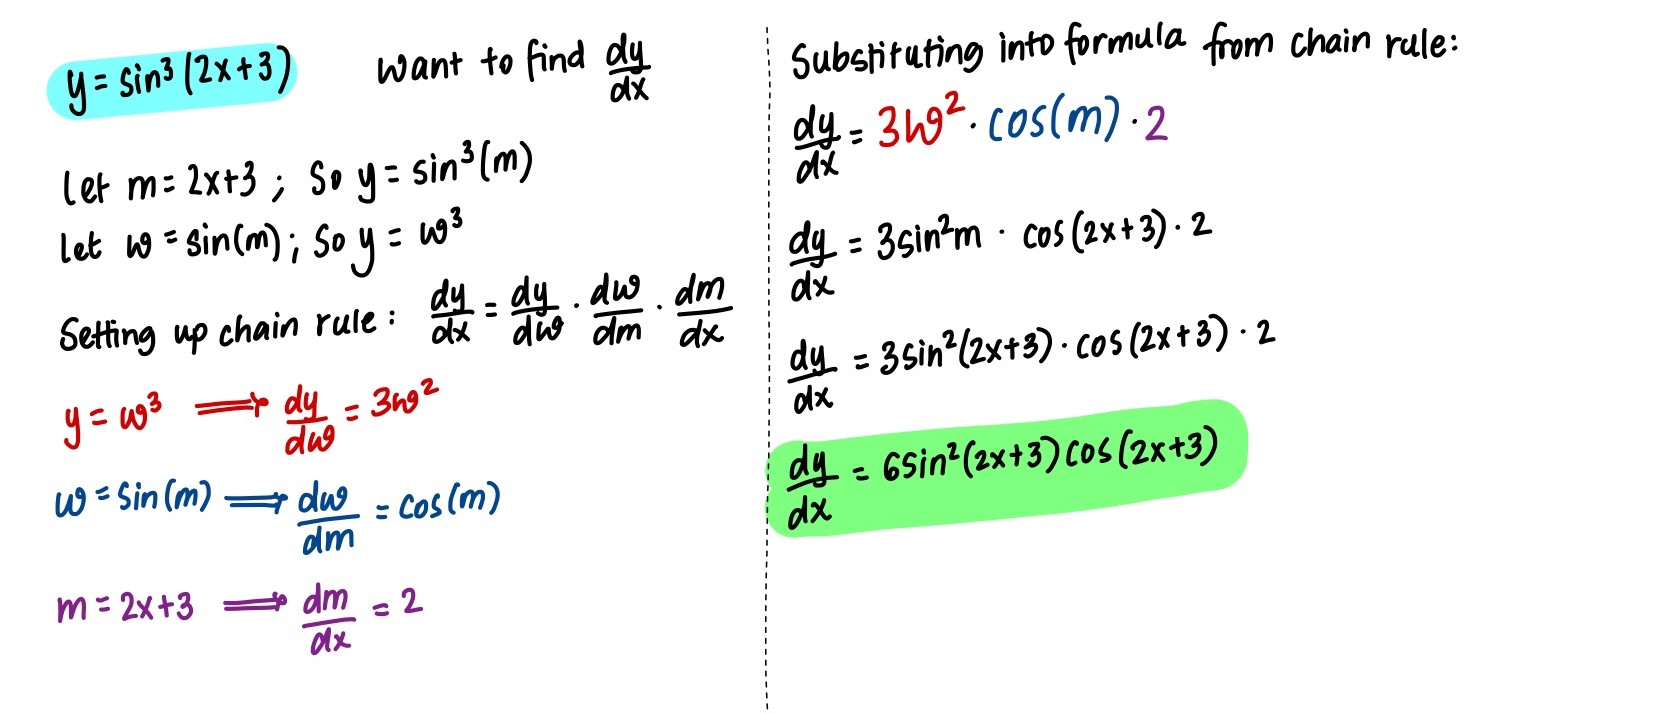
\includegraphics[width= \linewidth]{Q6.jpg}
        \label{fig:Q6}
    \end{figure}
\end{enumerate}

\subsection*{Product Rule}
Find the derivatives of the following functions (with respect to x):\\
\noindent \href{https://people.math.harvard.edu/~knill/teaching/math1a2021/handouts/lecture09.pdf}{Source} and another \href{https://math.arizona.edu/~calc/m124/Prod&Quot.pdf}{Source}

\begin{enumerate}
    \item $y = (x^8+2x-3)e^x$
    \begin{figure}[H]
        \centering
        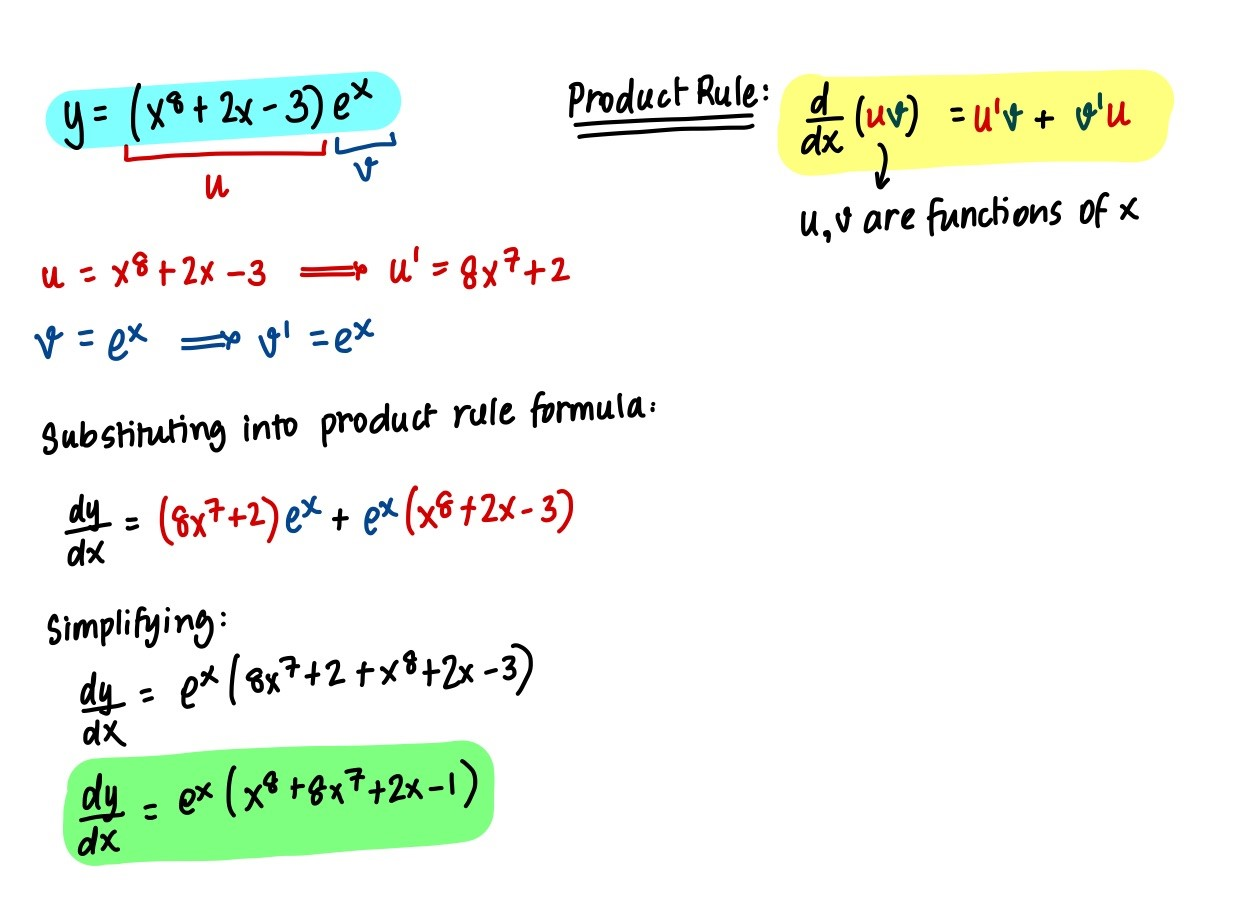
\includegraphics[width= 0.6\linewidth]{Q1.1.jpg}
        \label{fig:Q1.1}
    \end{figure}
    \item $y = 6xe^{2x}+8\tan3x$
    \begin{figure}[H]
        \centering
        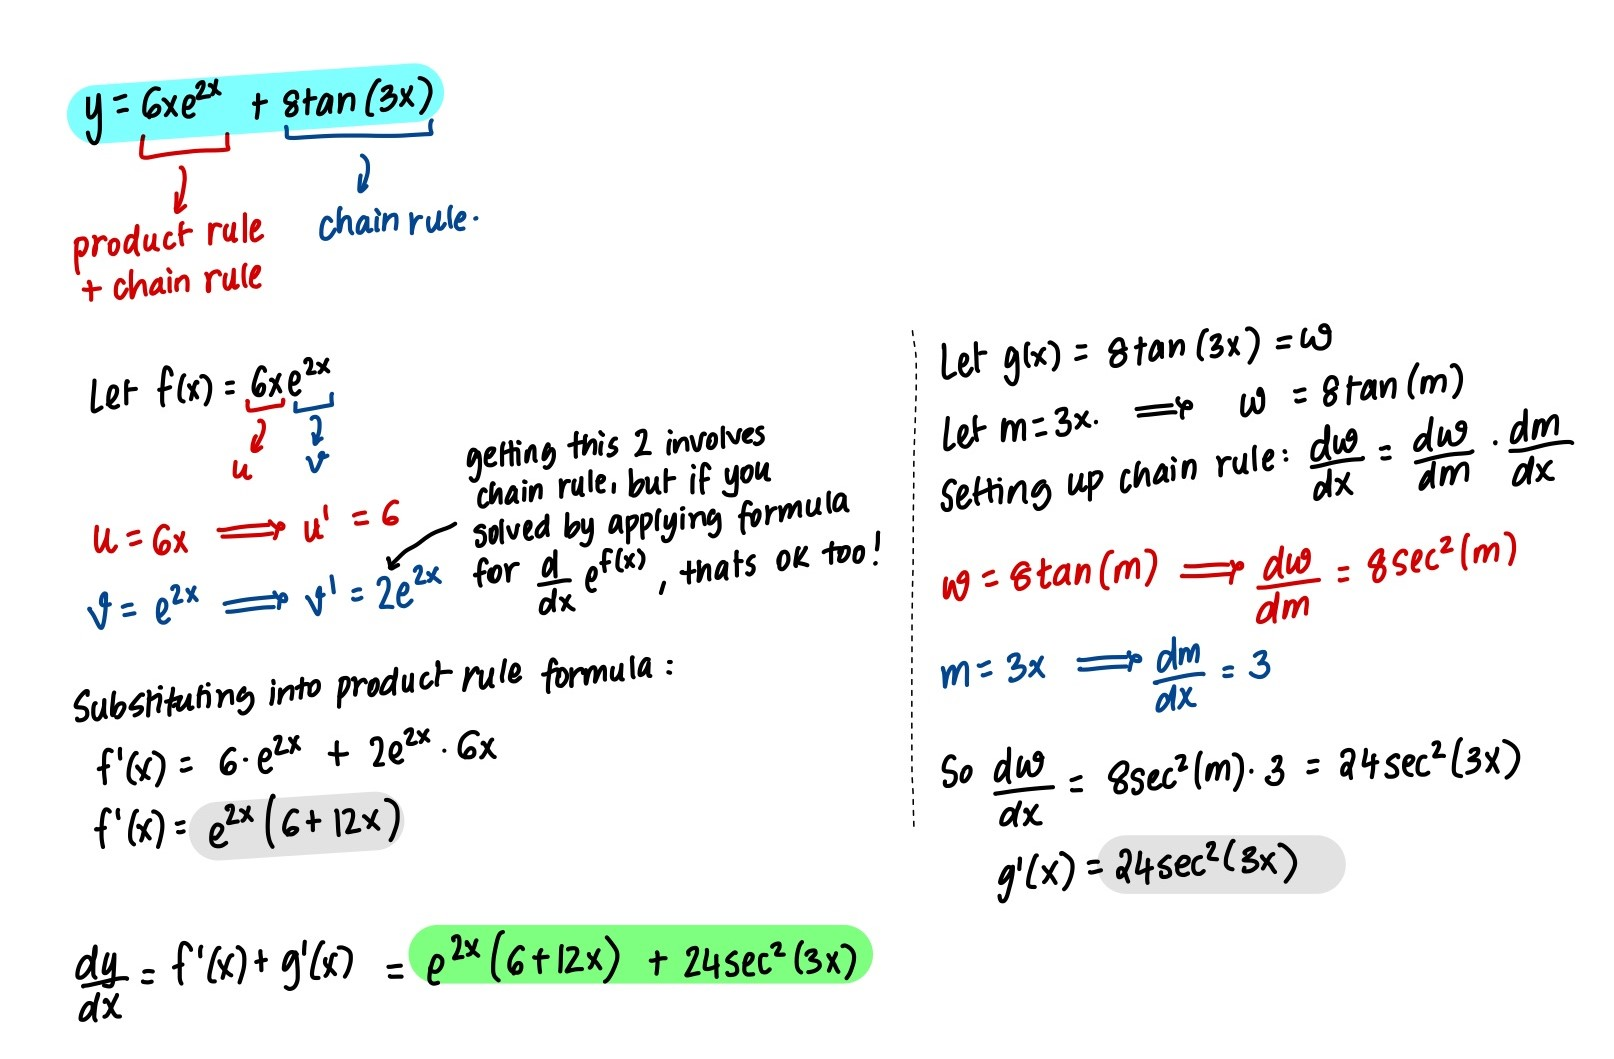
\includegraphics[width= 0.95\linewidth]{Q1.2.jpg}
        \label{fig:Q1.2}
    \end{figure}
    \item $y = 3e^x\sin x \cos x$
    \begin{figure}[H]
        \centering
        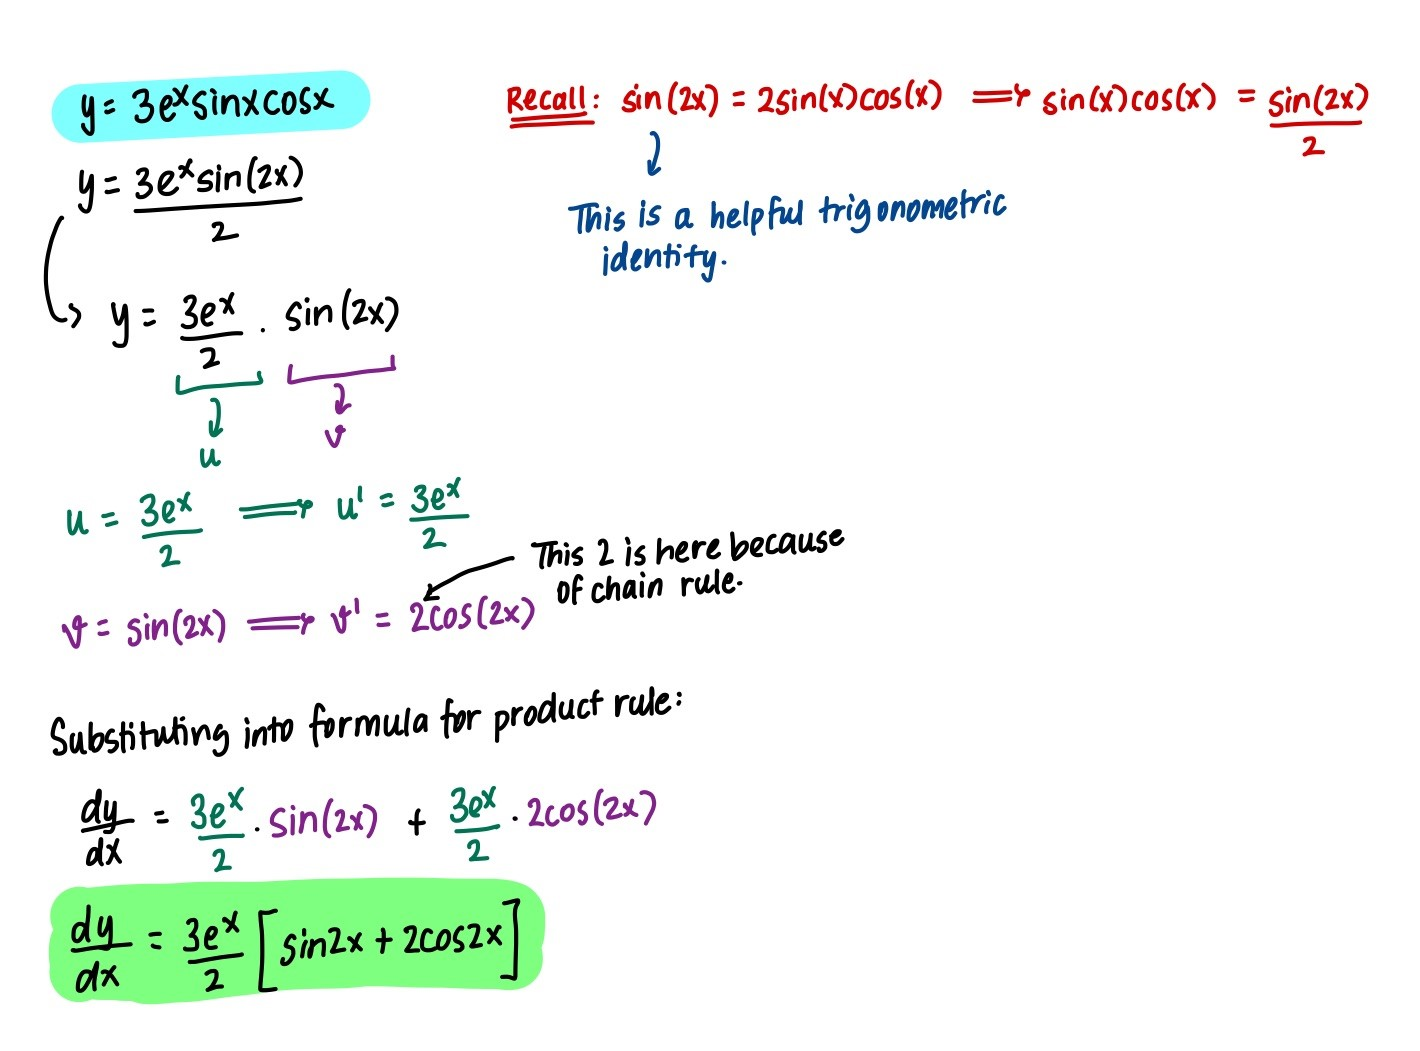
\includegraphics[width= 0.9\linewidth]{Q1.3.jpg}
        \label{fig:Q1.3}
    \end{figure}
    \item $y = (x+\sqrt{x})(3^x)$
    \begin{figure}[H]
        \centering
        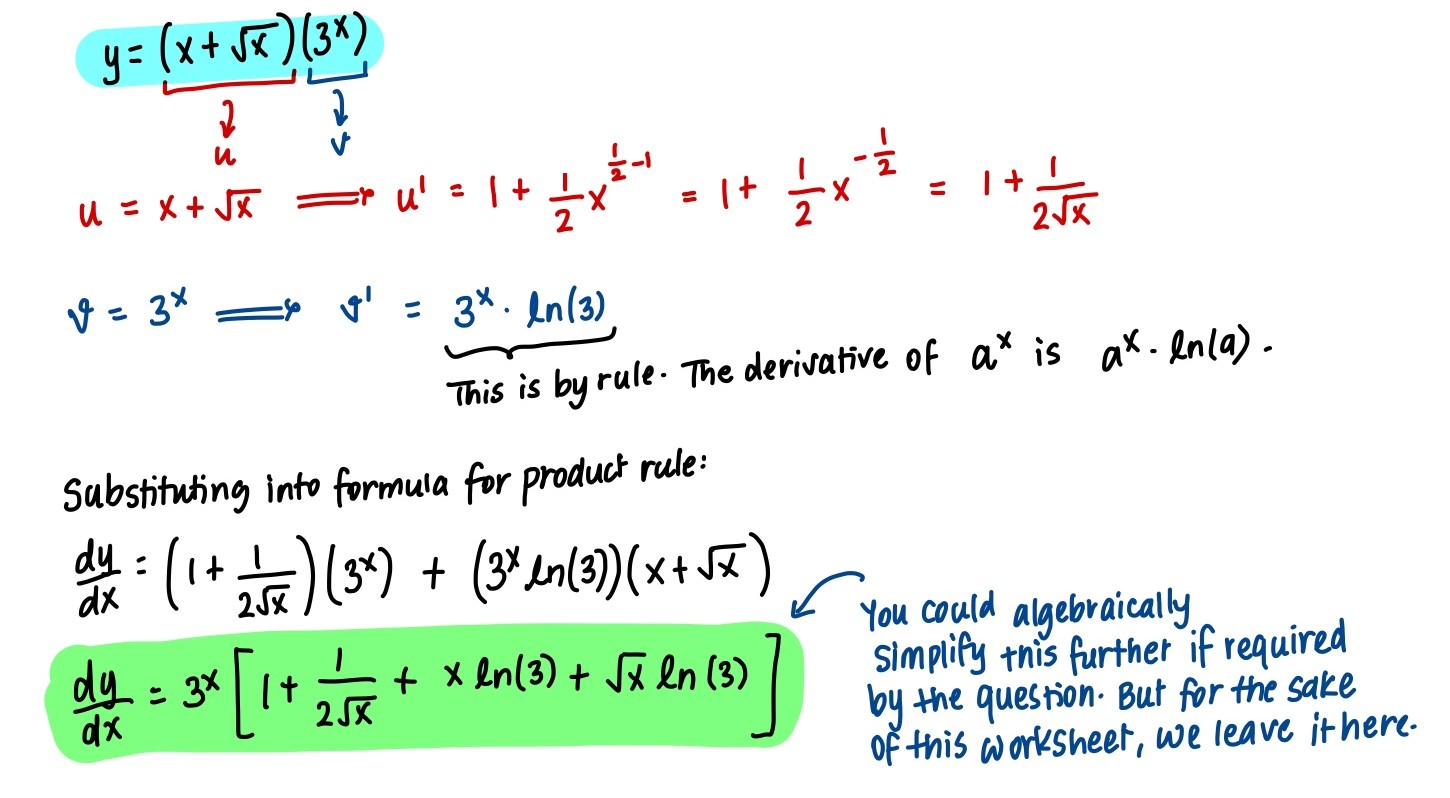
\includegraphics[width= 0.9\linewidth]{Q1.4.jpg}
        \label{fig:Q1.4}
    \end{figure}
\end{enumerate}

\subsection*{Quotient Rule}
Find the derivatives of the following functions (with respect to x):\\
\noindent \href{https://web.auburn.edu/holmerr/1617/Textbook/productquotient-screen.pdf}{Source}

\begin{enumerate}
    \item $f(x) = \frac{4 \cos(x) - 1}{2+3e^x}$
    \begin{figure}[H]
        \centering
        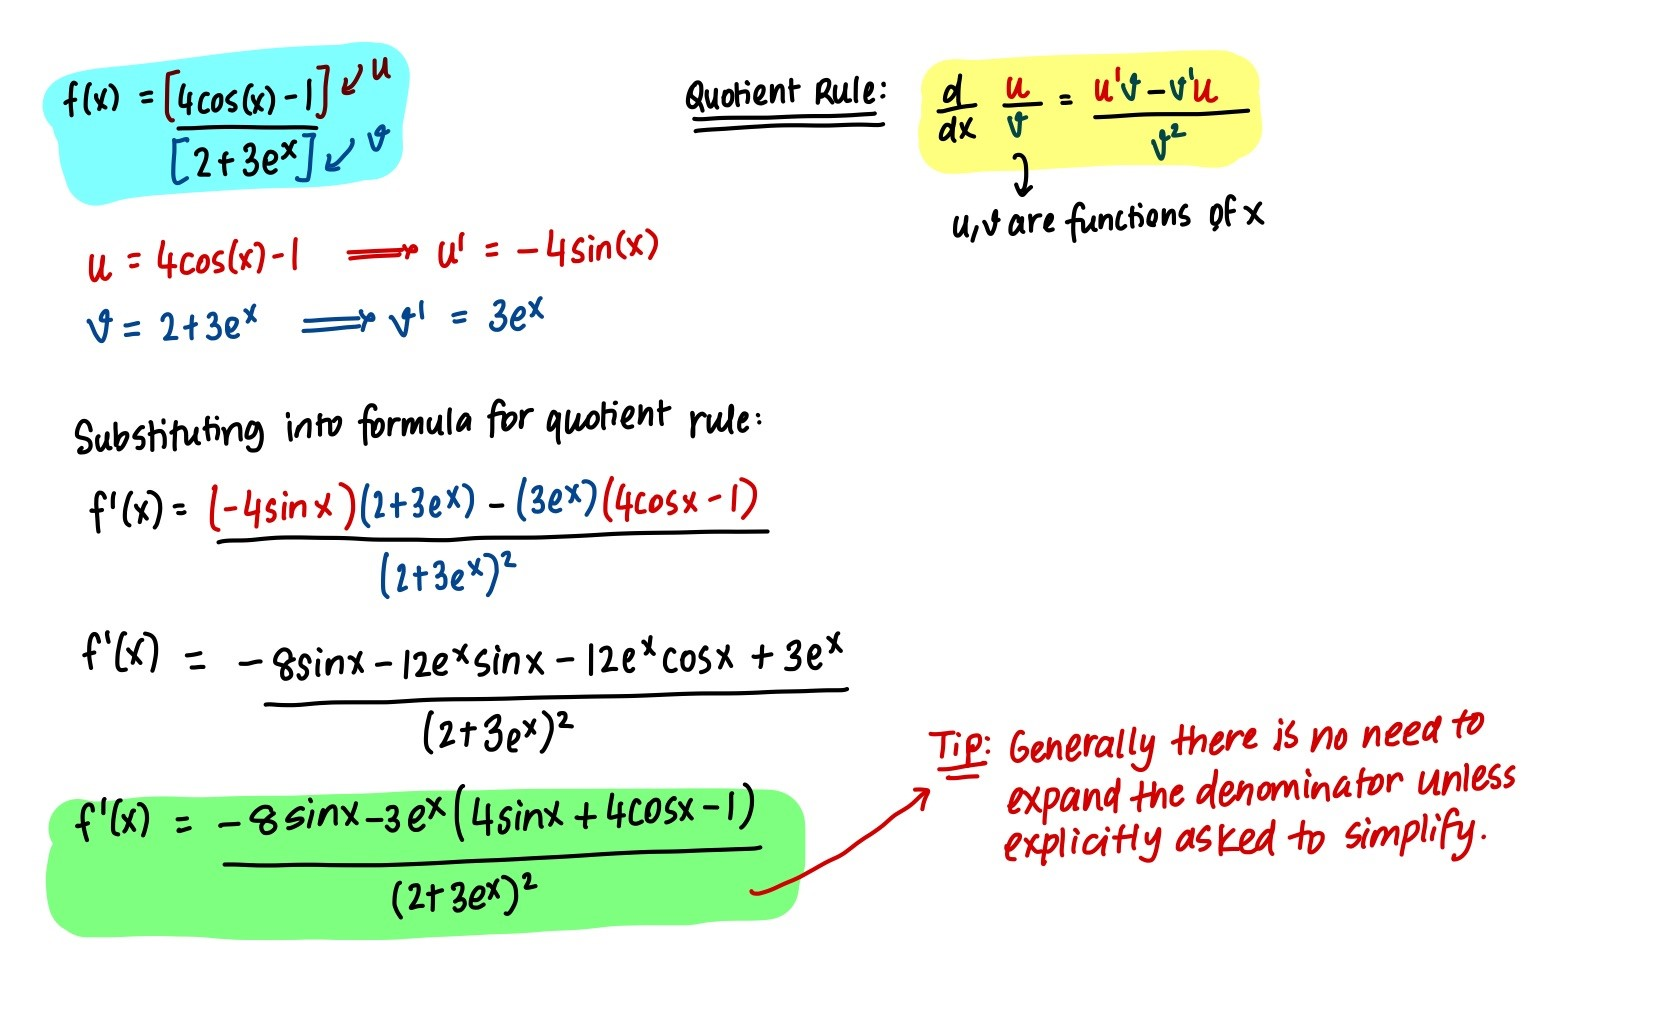
\includegraphics[width= 0.9\linewidth]{Q2.1.jpg}
        \label{fig:Q2.1}
    \end{figure}
    \item $y = \frac{3x^2}{5x-7}$
    \begin{figure}[H]
        \centering
        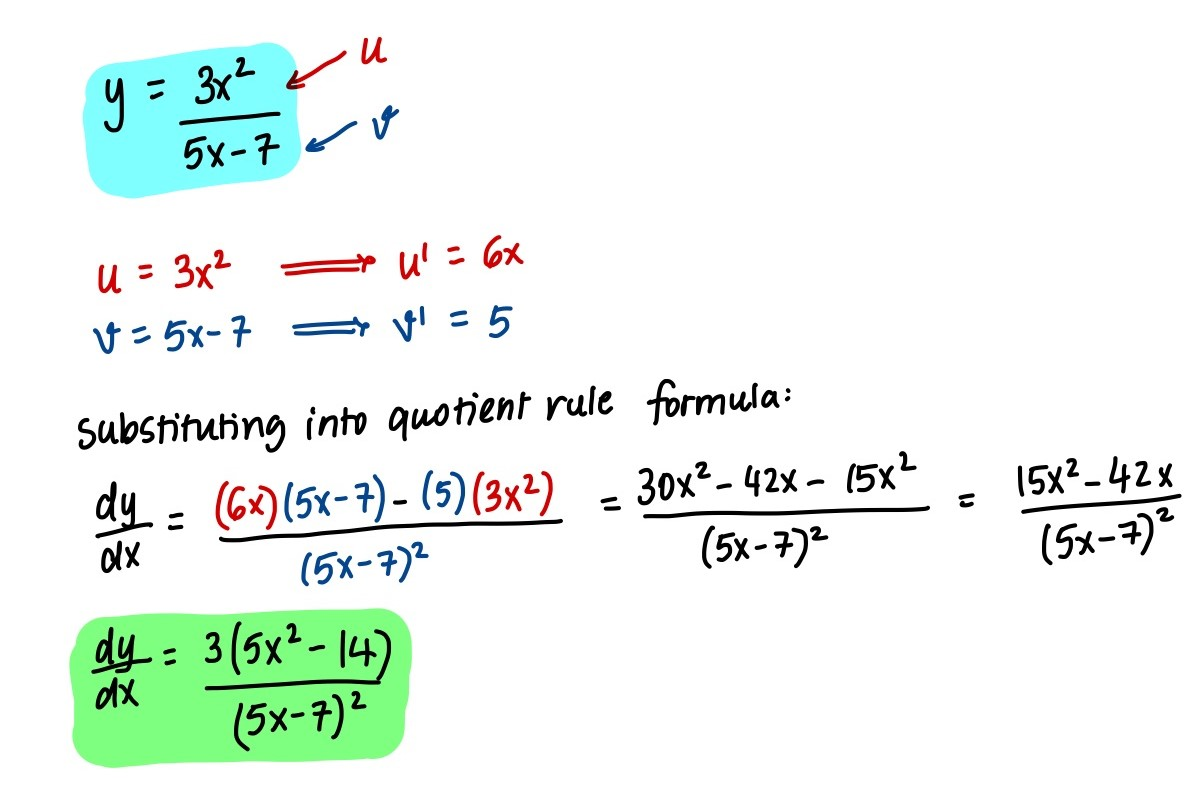
\includegraphics[width= 0.7\linewidth]{Q2.2.jpg}
        \label{fig:Q2.2}
    \end{figure}
    \item $y = \frac{e^x}{1+x}$
    \begin{figure}[H]
        \centering
        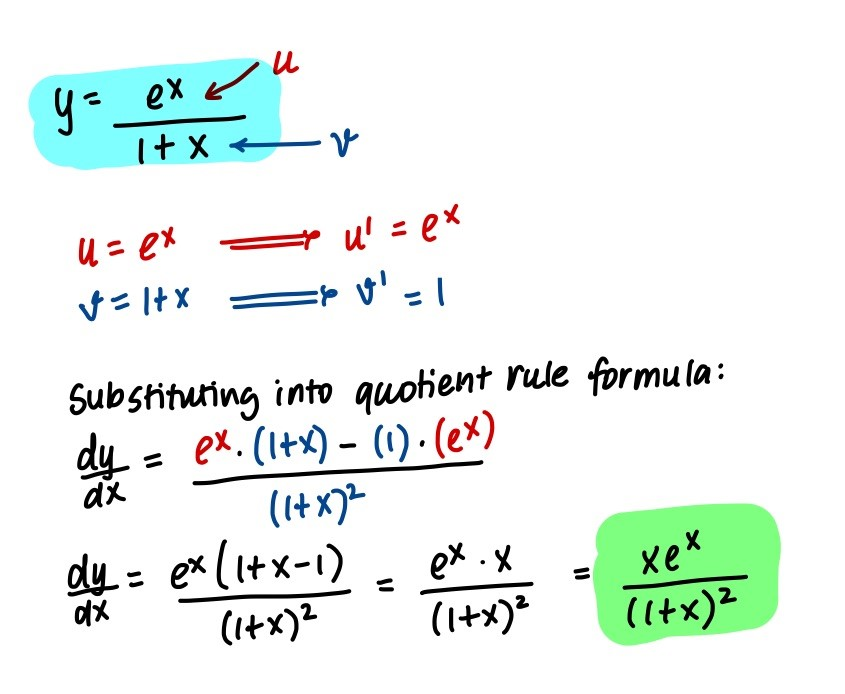
\includegraphics[width= 0.7\linewidth]{Q2.3.jpg}
        \label{fig:Q2.3}
    \end{figure}
    \item $y = \frac{\sin x}{x^2}$
    \begin{figure}[H]
        \centering
        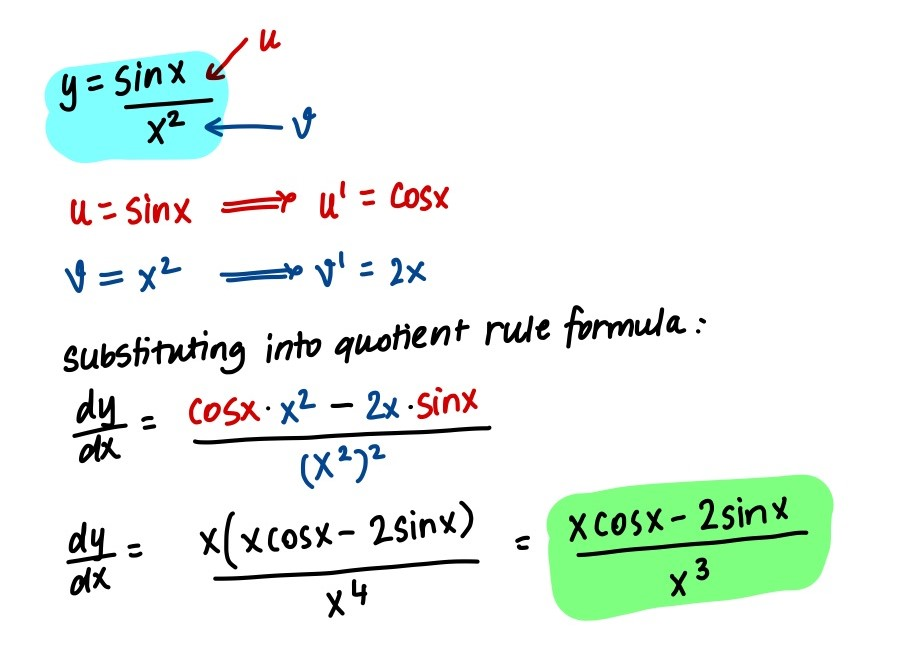
\includegraphics[width= 0.7\linewidth]{Q2.4.jpg}
        \label{fig:Q2.4}
    \end{figure}
\end{enumerate}

\end{document}
